%%%%%%%%%%%%%%%%%%%%%%%%%%%%%%%%%%%%%%%%%%%%%%%%%%%%%%%%%%%%%%%%%%%%%%%
% BAB 4
%%%%%%%%%%%%%%%%%%%%%%%%%%%%%%%%%%%%%%%%%%%%%%%%%%%%%%%%%%%%%%%%%%%%%%%

\mychapter{4}{BAB 4 METODOLOGI PELAKSANAAN PKL}

\section{Diagram Alir Metode}

Metode pelaksanaan Praktik Kerja Lapangan sebagai \textit{Technical Engineer}
pada APIE Pilot Project dilakukan melalui beberapa tahapan yang saling
berkaitan. Tahapan tersebut meliputi identifikasi kebutuhan jaringan pelatihan,
\textit{site survey}, analisis hasil survey, perancangan jaringan Wi-Fi,
persiapan perangkat AP dan WLC, implementasi dan konfigurasi, serta pengujian.
Alur pelaksanaan secara keseluruhan ditunjukkan pada Gambar~\ref{fig:diagram_alur_pkl}.

Apabila hasil pengujian belum sesuai dengan kebutuhan yang telah ditentukan,
dilakukan \textit{troubleshooting} untuk mengidentifikasi dan menangani
permasalahan yang ditemukan. Setelah permasalahan ditangani, dilakukan
pengujian ulang hingga perangkat dan skenario yang dipersiapkan memenuhi
kebutuhan pelatihan. Tahapan kemudian dilanjutkan dengan evaluasi sebagai
dasar dalam pengambilan kesimpulan.

\begin{figure}[H]
    \centering
    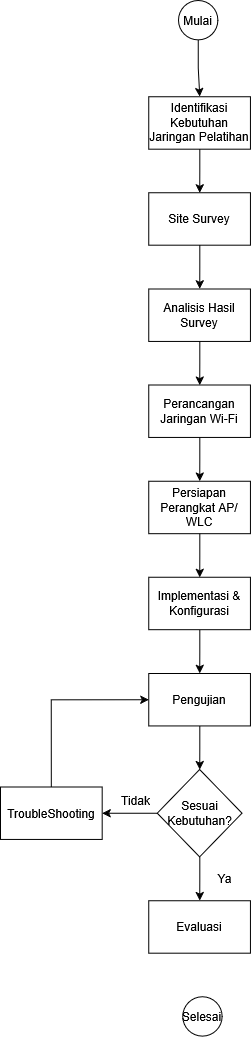
\includegraphics[
        height=0.7\textheight,
        keepaspectratio
    ]{img/Diagram-Alur-PKL.png}
    \caption{Diagram Alir Metode Pelaksanaan PKL}
    \label{fig:diagram_alur_pkl}
\end{figure}


\section{Spesifikasi Hardware dan Software}

\subsection{Hardware}

\begin{table}[H]
\centering
\caption{Hardware yang Digunakan}
\label{tab:hardware}
\begin{tabular}{|p{4cm}|p{10cm}|}
\hline
\textbf{Nama Perangkat} & \textbf{Fungsi} \\ \hline
Ruckus R550 & Menyediakan akses jaringan Wi-Fi pada lingkungan pelatihan. \\ \hline
H3C Switch & Menghubungkan perangkat jaringan pada lingkungan pelatihan. \\ \hline
\end{tabular}
\end{table}

\subsection{Software}

\begin{table}[H]
\centering
\caption{Software yang Digunakan}
\label{tab:software}
\begin{tabular}{|p{4cm}|p{10cm}|}
\hline
\textbf{Nama Software} & \textbf{Fungsi} \\ \hline
Omada Design Hub & Merancang jaringan Wi-Fi berdasarkan hasil site survey. \\ \hline
NetSpot & Melakukan site survey dan analisis kondisi jaringan Wi-Fi. \\ \hline
WSL & Menyediakan lingkungan Linux untuk kebutuhan teknis selama pelaksanaan. \\ \hline
Docker & Menjalankan layanan berbasis container yang digunakan dalam kegiatan. \\ \hline
RADIUS & Menyediakan layanan autentikasi untuk jaringan. \\ \hline
\end{tabular}
\end{table}


\section{Metode Perancangan}

Metode perancangan dilakukan untuk menghasilkan rancangan jaringan \textit{wireless} 
yang dapat digunakan sebagai referensi dalam pelaksanaan pelatihan APIE 
(\textit{Asia Pacific Internet Engineering}) Pilot Project di Gedung F Fakultas Ilmu 
Komputer Universitas Brawijaya. Perancangan difokuskan pada sisi jaringan \textit{wireless}, 
khususnya penempatan dan konfigurasi \textit{access point} (AP) yang dikelola melalui 
\textit{wireless LAN controller} (WLC). Rancangan dibuat berdasarkan kondisi jaringan 
\textit{wireless} yang telah tersedia pada lokasi kegiatan sehingga permasalahan pada 
kondisi \textit{existing} dapat digunakan sebagai dasar dalam menentukan rancangan yang 
lebih sesuai dengan kebutuhan pelatihan.

Tahap awal dilakukan dengan melakukan \textit{site survey} pada area Gedung F yang 
akan digunakan sebagai lokasi pelaksanaan kegiatan. \textit{Site survey} dilakukan 
untuk memperoleh gambaran kondisi jaringan \textit{wireless} pada lingkungan aktual, 
terutama terkait cakupan sinyal dan kondisi kanal yang digunakan. Hasil pengukuran 
kemudian dianalisis untuk mengidentifikasi kondisi jaringan yang perlu diperhatikan 
dalam perancangan, seperti area dengan cakupan sinyal yang belum memadai dan penggunaan 
kanal yang berpotensi menimbulkan \textit{overlap}.

Berdasarkan hasil analisis tersebut, dilakukan perancangan jaringan \textit{wireless} 
usulan menggunakan Omada Design Hub. Perancangan dilakukan dengan menentukan penempatan 
AP dan parameter jaringan \textit{wireless} yang diperlukan untuk menghasilkan cakupan 
dan konfigurasi kanal yang lebih sesuai dengan kebutuhan area pelatihan. Perancangan 
dilakukan pada lingkungan desain dan tidak mengubah konfigurasi AP yang telah terpasang 
pada jaringan \textit{existing}. Dengan demikian, rancangan yang dihasilkan merupakan 
rancangan usulan yang menggambarkan kondisi jaringan yang dapat digunakan sebagai 
referensi dalam kegiatan pelatihan.

Hasil dari tahap perancangan berupa \textit{reference wireless design} untuk Gedung F 
yang selanjutnya digunakan sebagai acuan dalam pelaksanaan skenario praktikum. 
Rancangan tersebut menjadi referensi bagi peserta dalam memahami proses perancangan 
dan deployment jaringan \textit{wireless} serta menjadi dasar untuk tahap implementasi 
dan pengujian yang dibahas pada bagian selanjutnya.

\section{Metode Implementasi}

Metode implementasi dilakukan untuk menerapkan kebutuhan dan rancangan jaringan
\textit{wireless} yang telah ditentukan pada tahap sebelumnya ke dalam lingkungan
pelatihan APIE Pilot Project. Implementasi difokuskan pada perangkat \textit{wireless}
yang menjadi ruang lingkup pekerjaan, yaitu \textit{access point} (AP) dan
\textit{wireless LAN controller} (WLC). Tahap ini dilakukan melalui persiapan,
konfigurasi, dan verifikasi perangkat sebelum kegiatan, kemudian dilanjutkan dengan
pendampingan teknis selama pelaksanaan \textit{hands-on}.

Pada tahap persiapan, dilakukan eksplorasi terhadap perangkat AP dan WLC untuk
memahami fungsi, antarmuka, serta konfigurasi yang diperlukan dalam skenario
pelatihan. Kegiatan eksplorasi dilakukan sebelum pelaksanaan agar perangkat yang
digunakan dapat dipahami dan dipersiapkan sesuai dengan kebutuhan skenario. Selanjutnya,
konfigurasi perangkat dilakukan berdasarkan kebutuhan masing-masing skenario dan
rancangan jaringan \textit{wireless} yang telah disiapkan. Setelah konfigurasi
diterapkan, dilakukan pemeriksaan terhadap kondisi perangkat dan konektivitas untuk
memastikan lingkungan pelatihan siap digunakan.

Pada saat pelaksanaan kegiatan, implementasi jaringan dilakukan oleh peserta
berdasarkan skenario dan \textit{worksheet} yang telah disiapkan. Penulis berperan
sebagai \textit{technical engineer} yang memberikan pendampingan teknis kepada
peserta selama proses implementasi. Pendampingan dilakukan dengan memberikan
penjelasan konfigurasi, membantu peserta ketika mengalami kendala, serta melakukan
\textit{troubleshooting} terhadap permasalahan yang muncul selama proses
\textit{hands-on}. Pendampingan dilakukan tanpa mengambil alih proses implementasi
yang menjadi bagian dari tugas peserta.

Setelah setiap sesi selesai, dilakukan pemeriksaan terhadap hasil pekerjaan yang
dikumpulkan serta identifikasi terhadap kendala teknis yang ditemukan selama
pelaksanaan. Temuan tersebut digunakan sebagai bahan evaluasi untuk melakukan
perbaikan atau persiapan teknis pada sesi berikutnya. Dengan demikian, metode
implementasi mencakup proses persiapan perangkat sebelum kegiatan dan dukungan
teknis selama pelaksanaan untuk memastikan skenario jaringan dapat digunakan sesuai
dengan kebutuhan pelatihan.

\section{Metode Pengujian}

Metode pengujian dilakukan untuk memverifikasi bahwa perangkat dan skenario jaringan
\textit{wireless} yang dipersiapkan dapat berfungsi sesuai dengan kebutuhan pelatihan.
Pengujian dilakukan terhadap perangkat yang menjadi ruang lingkup teknis, yaitu
\textit{access point} (AP) dan \textit{wireless LAN controller} (WLC), serta terhadap
skenario yang digunakan selama pelaksanaan kegiatan.

Pengujian diawali dengan pemeriksaan fungsi perangkat dan konfigurasi yang telah
diterapkan. Pemeriksaan dilakukan untuk memastikan AP dapat terhubung dan dikelola
melalui WLC serta konfigurasi jaringan yang diperlukan dapat diterapkan. Selanjutnya,
dilakukan pengujian konektivitas untuk memastikan perangkat dan layanan jaringan yang
digunakan pada skenario dapat saling terhubung sesuai dengan kebutuhan.

Setelah fungsi dan konektivitas perangkat terpenuhi, dilakukan validasi terhadap
skenario pelatihan dengan menjalankan langkah-langkah yang terdapat pada
\textit{worksheet} atau \textit{mission card}. Validasi dilakukan dengan memeriksa
apakah setiap tahapan pada skenario dapat dijalankan dan menghasilkan kondisi yang
diharapkan. Apabila ditemukan kendala selama pengujian, dilakukan identifikasi
permasalahan dan \textit{troubleshooting}, kemudian pengujian diulangi untuk
memastikan permasalahan telah terselesaikan.

Hasil dari proses pengujian digunakan untuk menentukan kesiapan perangkat dan
skenario sebelum digunakan dalam kegiatan pelatihan. Temuan yang diperoleh selama
pengujian juga digunakan sebagai bahan evaluasi dan persiapan teknis untuk sesi
berikutnya.

\section{Metode Pengambilan Kesimpulan}

Metode pengambilan kesimpulan dilakukan dengan mengevaluasi hasil implementasi dan
pengujian terhadap kebutuhan jaringan \textit{wireless} yang telah ditentukan pada
tahap sebelumnya. Evaluasi dilakukan dengan membandingkan kondisi yang diperoleh dari
pelaksanaan dengan kondisi yang diharapkan pada masing-masing skenario.

Hasil pengujian kemudian dianalisis untuk menentukan apakah perangkat dan skenario
jaringan telah berfungsi sesuai dengan kebutuhan pelatihan. Apabila ditemukan
kendala, hasil \textit{troubleshooting} dan pengujian ulang turut dipertimbangkan
dalam proses evaluasi. Selain itu, temuan selama pelaksanaan digunakan untuk
mengidentifikasi aspek teknis yang masih memerlukan perbaikan atau persiapan lebih
lanjut.

Berdasarkan hasil evaluasi tersebut, kesimpulan disusun untuk menjawab rumusan
masalah mengenai proses implementasi dan hasil pengujian skenario jaringan Wi-Fi
pada APIE Pilot Project Universitas Brawijaya.